\chapter{Experimental Methods}
%Os experimentos são descritos aqui. 
In order to compare experimental results with the theoretical prevision we must measured two parameters in the Eq.\ref{eq:taxa_ir_broad} and \ref{eq:taxa_vis_broad}. First we need to characterize the visible mode by measure the losses $\kappa^(i)_3$ and $\kappa^(e)_3$; we have apply two different, and complementary, techniques for that. The second important parameter is the Coupling terms $B_1$ and $B_3$; the challenge lays in the calculation of the overlap integral, as defined in Eq~\ref{eq:overlap_j3}. With this values in hand, we must be able to compare the theoretical and experimental results. 

But first of all, the main experiment in this dissertation is the generation of third harmonic in optical microcavities. Lets star by there. %This Chapter present a scientific description of the experiments, meanwhile a technical overview is presented in the Appendix~\ref{app:experiment}

\section{Third Harmonic Generation in Optical Microcavities}

The experiment is done with a setup quite similar to the one used in the optical characterization of infrared modes, show in Fig~\subref{fig:exp_mode_charac}{a}, with the inclusion of a wave modulator, a Erbium Doped Fiber Amplifier and a free space setup in the output to split the infrared (which was high powered) from the third harmonic.
\begin{figure}[h!]
    \centering
    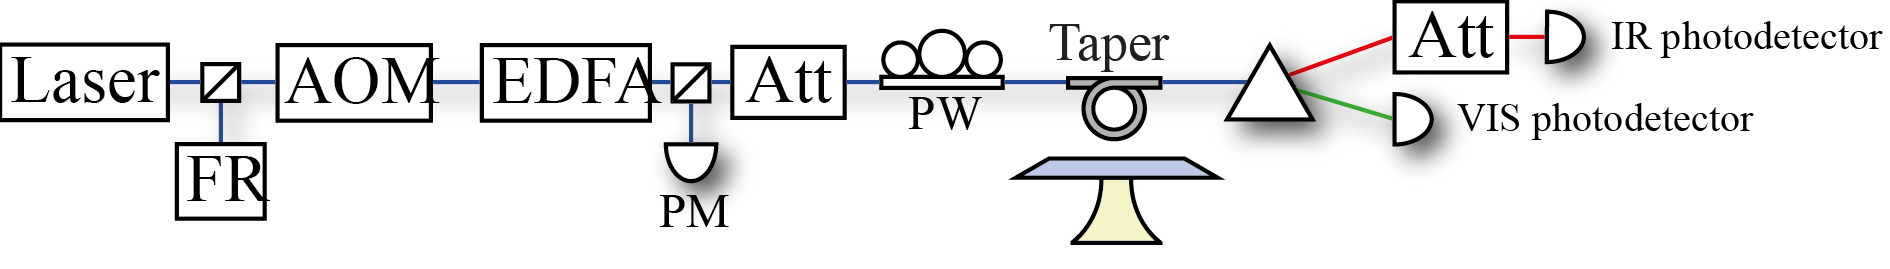
\includegraphics[width = 16 cm]{figuras/Dissertation_thg_setup.jpg}
    \caption{\textbf{Experimental Setup:} A infrared tunable Laser is modulated by a Acousto-optic Modulator (AOM) and amplified by a Erbium Doped Fiber Amplifier (EDFA) up to tens of watts. A Frequency Reference (FR) is used to precisely determine the frequency of the source, attenuator (att.) and paddle wheels are used to control the input power and polarization. The infrared part is splitted from the visible by a prism.}
    \label{fig:thg_setup}
\end{figure}

As seen in Chapter~\ref{chap:nonlin_pol}, to observe third order effects it is needed a power higher than the used in transmission experiment. To reach power high enough a Erbium Doped Fiber Amplifier is applied, which amplifies the optical power to around $40$ dBm. Beside the EDFA, the input wave is modulated in pulses with width of $400$~ns and duty cycle of $40$~$\mu$s using a Acousto-optic Modulator. The working principle of the EDFA makes the mean power to keep constant, leading to higher peak power. In this dissertation we have reach peak power around $4$~W.  

The amplified power is monitored using a beam splitter. A fentosecond detector able to solve the pulse format enables to measured the power in function of time with the aid of a oscilloscope. The input power is controlled using a Attenuator, to keep the power measured by the IR photodetector at constant range another Attenuator is add to the circuit, the sum of the attenuation in both is keep constant.  

The experiment is done by sweep the frequency of the source and monitoring the power at the VIS photodetector. The result of the experiment is the power in visible in function of the frequency of the source, as show in Fig.~\ref{fig:thg_broad_map}, each peak corresponds to a scenario wheres the condition to third harmonic generations, as sens in Chapter~\ref{chap:couple_mode}, was satisfied; this result was preliminary obtained with the initial defective wafer. 
\begin{figure}[h]
    \centering
    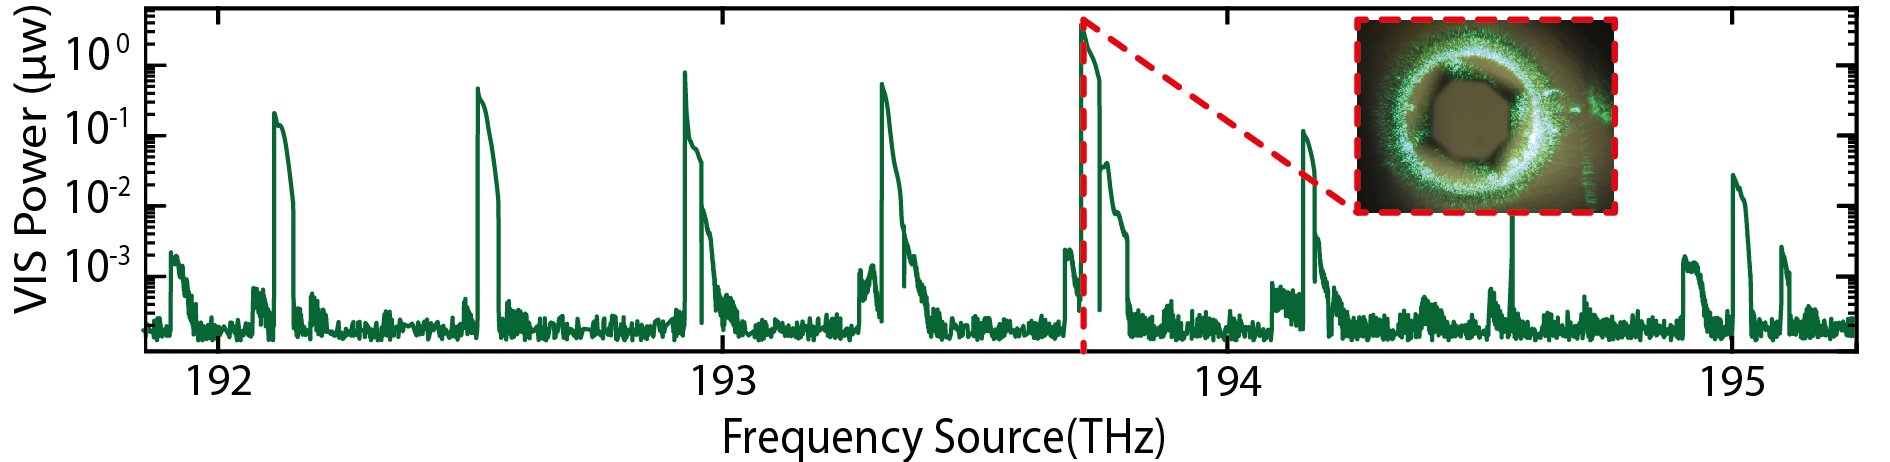
\includegraphics[width = 16cm]{figuras/Dissertation_thg_broad.jpg}
    \caption{Collected visible light in function of the source frequency. Insert of an actual picture of a cavity emitting Third Harmonic.}
    \label{fig:thg_broad_map}
\end{figure}

The shape of the THG curves is significantly different of those predicted in the Fig.~\ref{fig:temporal_solution}, this is due to the interference between neighboring infrared modes. As the coupling between the cavity and the source must be high in in order to collect more TH, the amount of excited IR modes is high enough to produce a dirty transmission spectrum. 

Now we are interested in control the phase matching condition between the modes by change the phase detuning $\delta_\omega$. To change the phase detuning we shall vary the sample temperature, which gives rise to a dynamics similar to the presented in the Eq~\ref{eq:termooptc_change}, but with a external heat source instead of internal one, enabling to rewrite the Eq~\ref{eq:pertubation_bistaliti_cavity} can by write as 
\begin{equation}
    \frac{\Delta\omega_\alpha}{\omega_\alpha} = \frac{d\text{n}_\alpha}{dt}\Delta T \rightarrow \Delta\delta_\omega = \left(\omega_3\frac{d\text{n}_3}{dt} - 3\omega_1\frac{d\text{n}_1}{dt}\right)\Delta T
    \label{eq:temperature_mode_variation}
\end{equation}
the frequency displacement due to the sample temperature is different for each band, leading to a variation in the initial phase detuning. Then it is possible to calculate the variation in the phase detuning in function of the temperature and compare the effect over the third harmonic generation. 

The experimental result can be quantitatively compared with the numerical solution of the Eq~\ref{eq:taxa_ir_broad} and Eq~\ref{eq:taxa_vis_broad} for different values of $\delta\omega$. The result is presented in Fig.~\ref{fig:thg_control_phase_det}. This measurement was made with a increase in the diameter of the tapered fiber, in relation with the Fig.~\ref{fig:thg_broad_map}, cleaning the infrared spectrum; however, it decrease the amount of collected visible power. Another important difference is the use of samples fabricated with lab grown wafer.
\begin{figure}[!h]
    \centering
    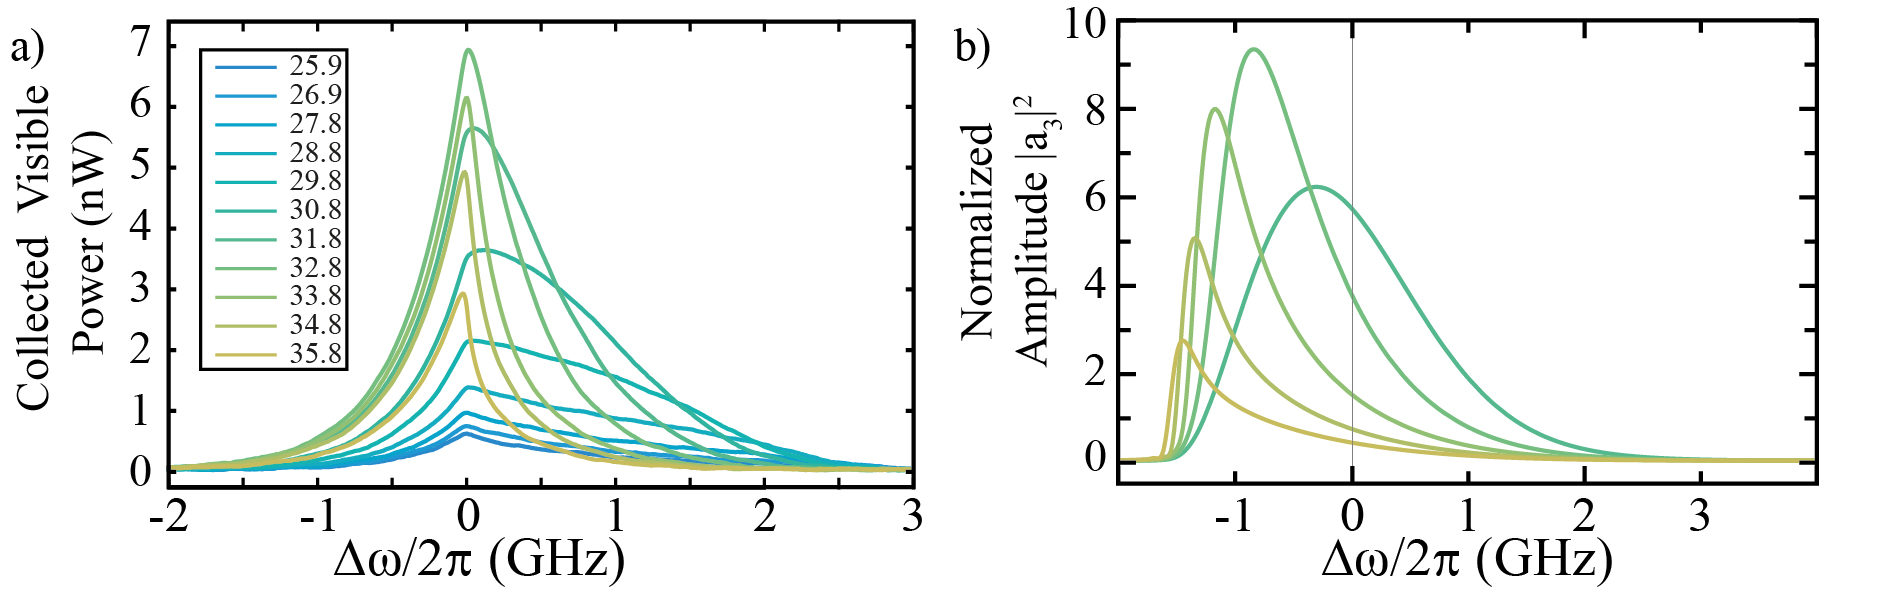
\includegraphics[width = 16cm]{Dissertation_phase_detuning_comp.jpg}
    \caption{\textbf{Model Comparison: a)} Collected visible light in function of the Detuning of the source with the infrared mode for different values of temperature, hence, different phase detuning. \textbf{b)} Simulated inner energy storage in the visible mode in function of the Detuning of the source with the infrared mode for different phase detuning. The curves was normalized by the same value.}
    \label{fig:thg_control_phase_det}
\end{figure}

In order to produce a quantitative comparation we need to measured the parameters cited above.  

\section{Optical Characterization at Visible Band}

The main challenge in characterize the cavity in the visible band is the lack of a tunable visible laser, which could be used as described in the Sections~\ref{sec:optical_char}. As we do not have access to a visible tunable laser, we need to apply a different techniques, two to be precise. One technique use the transmitted light from a external source, slightly similar from the infrared characterization, the other one use the emitted third harmonic. 

\subsection{Transmission Characterization}

This experiment is based on the Eq~\ref{eq:single_mode_transmission}, wheres the Detuning $\Delta_3$ (do not mistake with the phase detuning $\delta_\omega$) was defined $\Delta_3 = \omega_3 - \omega$. The source used was a visible green laser ($532$~nm) with fixed frequency ($\omega$); therefore, in order to compute the transmission spectrum we vary the resonance frequency $\omega_3$ by change the sample temperature, according with the Eq.~\ref{eq:temperature_mode_variation} we can write 
\begin{equation}
    \Delta_3 = \omega_3\frac{d\text{n}_3}{dT}\Delta T.
\end{equation}
To determine the $\Delta T$ an infrared mode was used as probe.

The Fig.~\ref{fig:mode_char_trans} shows the result of the experiment. An infrared mode was characterize using the same procedure, as shown in Fig.~\subref{fig:mode_char_trans}{b}, where we can calculate the losses, $\kappa_1^{(i)} = 940\pm 50$~MHz and $\kappa_1^{(e)} = 180 \pm 6$~MHz, them we compare with the typical characterization (as described in Chapter~\ref{chap:optical_cavity}), show in Fig.~\subref{fig:mode_char_trans}{a}, we have measured $\kappa_1^{(i)} = 910\pm 20$~MHz and $\kappa_1^{(e)} = 173 \pm 2$~MHz; both techniques are in well agreement for the infrared mode.
\begin{figure}[!h]
    \centering
    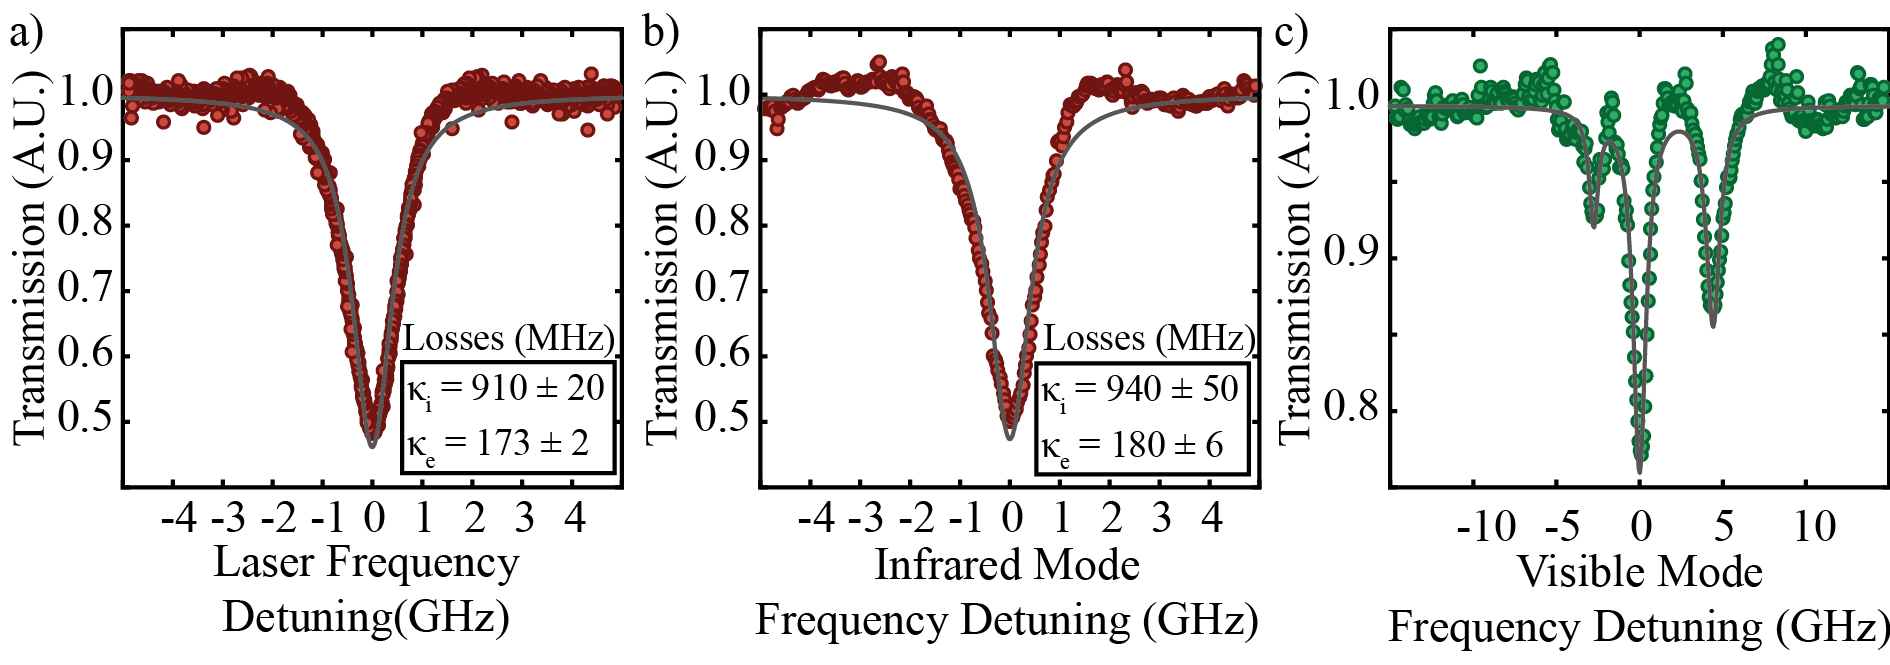
\includegraphics[width = 16cm]{Dissertation_char_vis_trans.jpg}
    \caption{\textbf{Transmission Characterization: a)} Infrared mode characterized using a tunable laser. \textbf{b)} Same infrared mode characterized using thermal shift. Both results are in well agreement. \textbf{c)} Characterization of the visible mode using thermal shift. }
    \label{fig:mode_char_trans}
\end{figure}

The results for the visible mode is shown in the Fig~\subref{fig:mode_char_trans}{c}. It was possible to identify three different modes, all of them  was fitted with a variation of the Eq~\ref{eq:single_mode_transmission} to include the neighbors~\needcit. We have found the values
\begin{table}[h]
\centering
\begin{tabularx}{8cm}{c|c|c|c}
Modo & $\kappa_i$ (MHz) & $\kappa_e$ (MHz) & $Q_i$ ($10^5$) \\ 
\hline                               
1 &$700\pm200$&$12\pm2$&$9.0\pm2.0$\\
2 &$870\pm60$&$59\pm3$&$6.6\pm0.4$\\
3 &$950\pm90$&$37\pm2$&$6.1\pm0.5$
\end{tabularx}
\caption{Losses and intrinsic Quality factor for the visible modes shown above}
\end{table}

It is important to notice that the measured modes are out of band where we have measured third harmonic as the fundamental mode for this visible modes lies around the $1596$~nm, out of the EDFA band; however, this result bring us a strong feeling about the coupling rate between the visible modes and the source. The bus waveguide was designed for coupling infrared modes, which lead to a poor coupling for visible mode, as demonstrated in the numerical solution, the amount of visible light collected is strong dependent on the coupling, this result explain the low collected power presented in the Fig.~\subref{fig:thg_control_phase_det}{a}.

This technique characterize both $\kappa_3^{(i)}$ and $\kappa_3^{(e)}$, although it do not characterize a mode that we can measure third harmonic. The next technique use the generation of third harmonic to measures the losses, so, we necessary will be looking for a mode the interest band, in exchange, it will only be possible to measure the total loss. 

\subsection{Third Harmonic Generation Characterization}

Lets introduce a set of assumptions in order to rewrite the Eq~\ref{eq:taxa_ir_broad} and \ref{eq:taxa_vis_broad}. First, consider the steady state, $\dot{a}_\alpha = 0$, also lets consider that the system is in the resonance of the infrared, $\Delta_1 = \omega_1(A_{11}|a_1|^2+A_{13}|a_3|^2)$ for last we assume that the $a_3$ amplitude is much smaller than $a_1$, then we can write the energy in the visible mode as
\begin{equation}
    |a_3|^2 = \frac{|\omega_3 B_3 (a_1)^3|^2}{\left(\kappa_3\right)^2 + \left(\delta_0 - 3(A_{31}-A_{11})|a_1|^2\right)^2}
    \label{eq:thg_phase_mismatch}
\end{equation}

The assumption of resonance with the infrared is important to consider all parameters independents of the phase detuning, which lead to a Lorentzian function for the energy stored in the visible mode with the phase detuning as variable. Using the same procedure as before to vary the phase detuning and measuring the third harmonic power generated in the resonance of infrared is possible to determine the total loss $\kappa_3$. The result is shown in the Fig.~\ref{fig:mode_char_thg}.
\begin{figure}[!h]
    \centering
    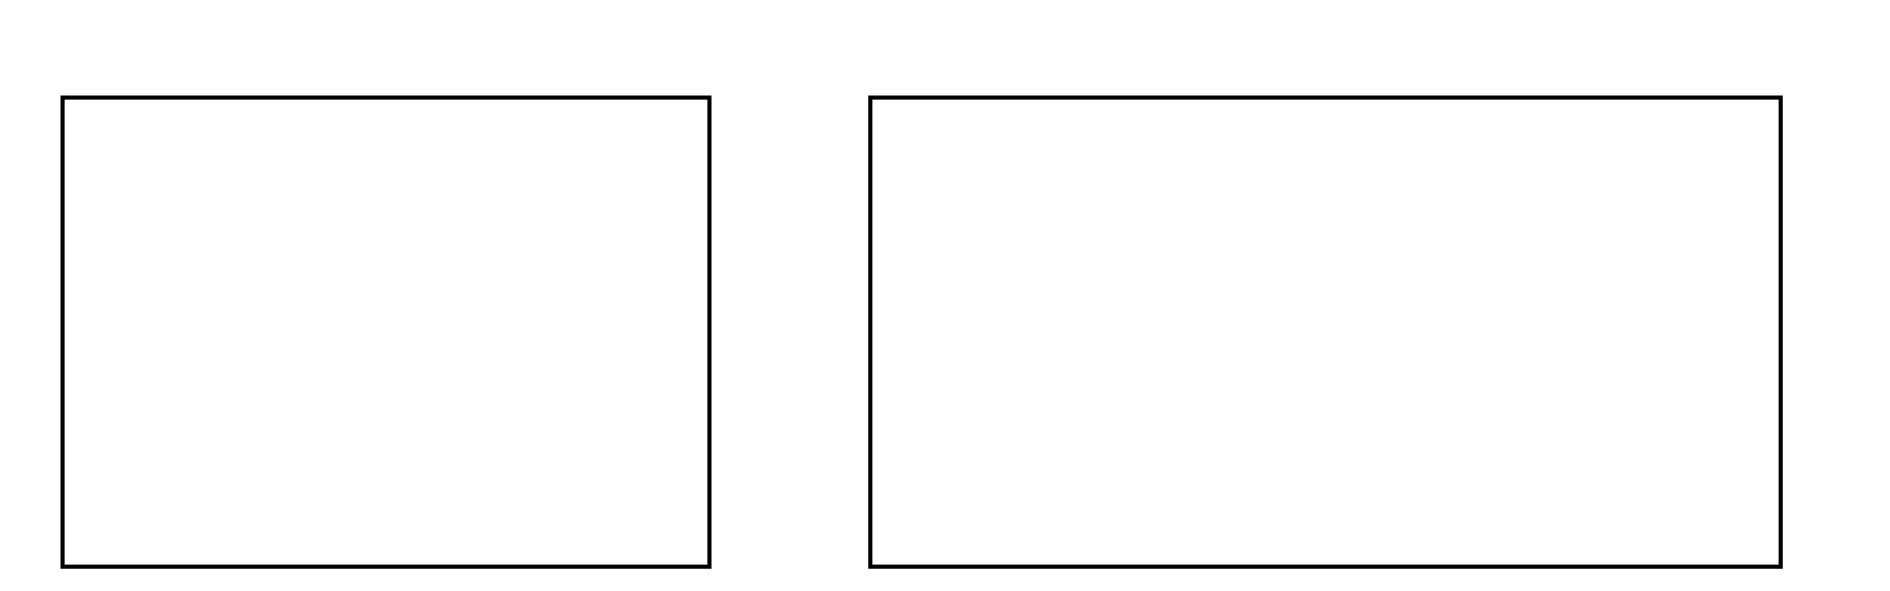
\includegraphics[width = 16cm]{Dissertation_char_vis_thg.jpg}
    \caption{\textbf{Visible Emission Characterization: a)} Infrared transmission and visible emission simultaneous measured in function of the source frequency for different temperatures, shown in the insert box, and a fixed power. The dashed lines mark the resonance frequency. Both data was normalized in order to facilitate the visualization. \textbf{b} Visible collected power (without the normalization) at the resonance frequency in function o the phase detuning for different input power,  shown in the insert box.}
    \label{fig:mode_char_thg}
\end{figure}

Fitting the result with the Eq.~\ref{eq:thg_phase_mismatch} we determined the total loss as $\kappa_3 = 592\pm13$~MHz, which is comparable with the results obtained by the transmission technique. Using the same rate between the coupling and the intrinsic loss, we can estimate the values $\kappa_3^{(i)} = 567\pm17$~MHz and $\kappa_3^{(e)}=25\pm10$~MHz. 

An natural conclusion is think that is possible to use the Eq.~\ref{eq:out_wave} simultaneously with Eq.\ref{eq:thg_phase_mismatch} to determine the coupling rate by fitting; however, the fit would calculate the whole numerator, in other word, the fit determine the value of $\kappa_3^{(e)}|\omega_3 B_3 (a_1)^3|^2$, to use this information to infer the coupling rate we must first know the Coupling term $B_3$ and the infrared mode amplitude $a_1$, both aren't possible to directly measure which makes this procedure complicated and fragile due to errors propagation. 

In order to get a reliable estimate we must determine the Coupling term. As already seen, this term depends on the spatial distribution of the mode, which can't be measured but is calculated using simulation.

\section{Coupling Term Estimation}

The coupling terms $B_1$ and $B_3$ can't be directly measured. One way to estimate their values is be simulate the both modes, using Finite Element Method, to determine the spatial distribution and calculate the overlap integral, Eq.\ref{eq:overlap_j3}.

\begin{figure}[t]
    \centering
    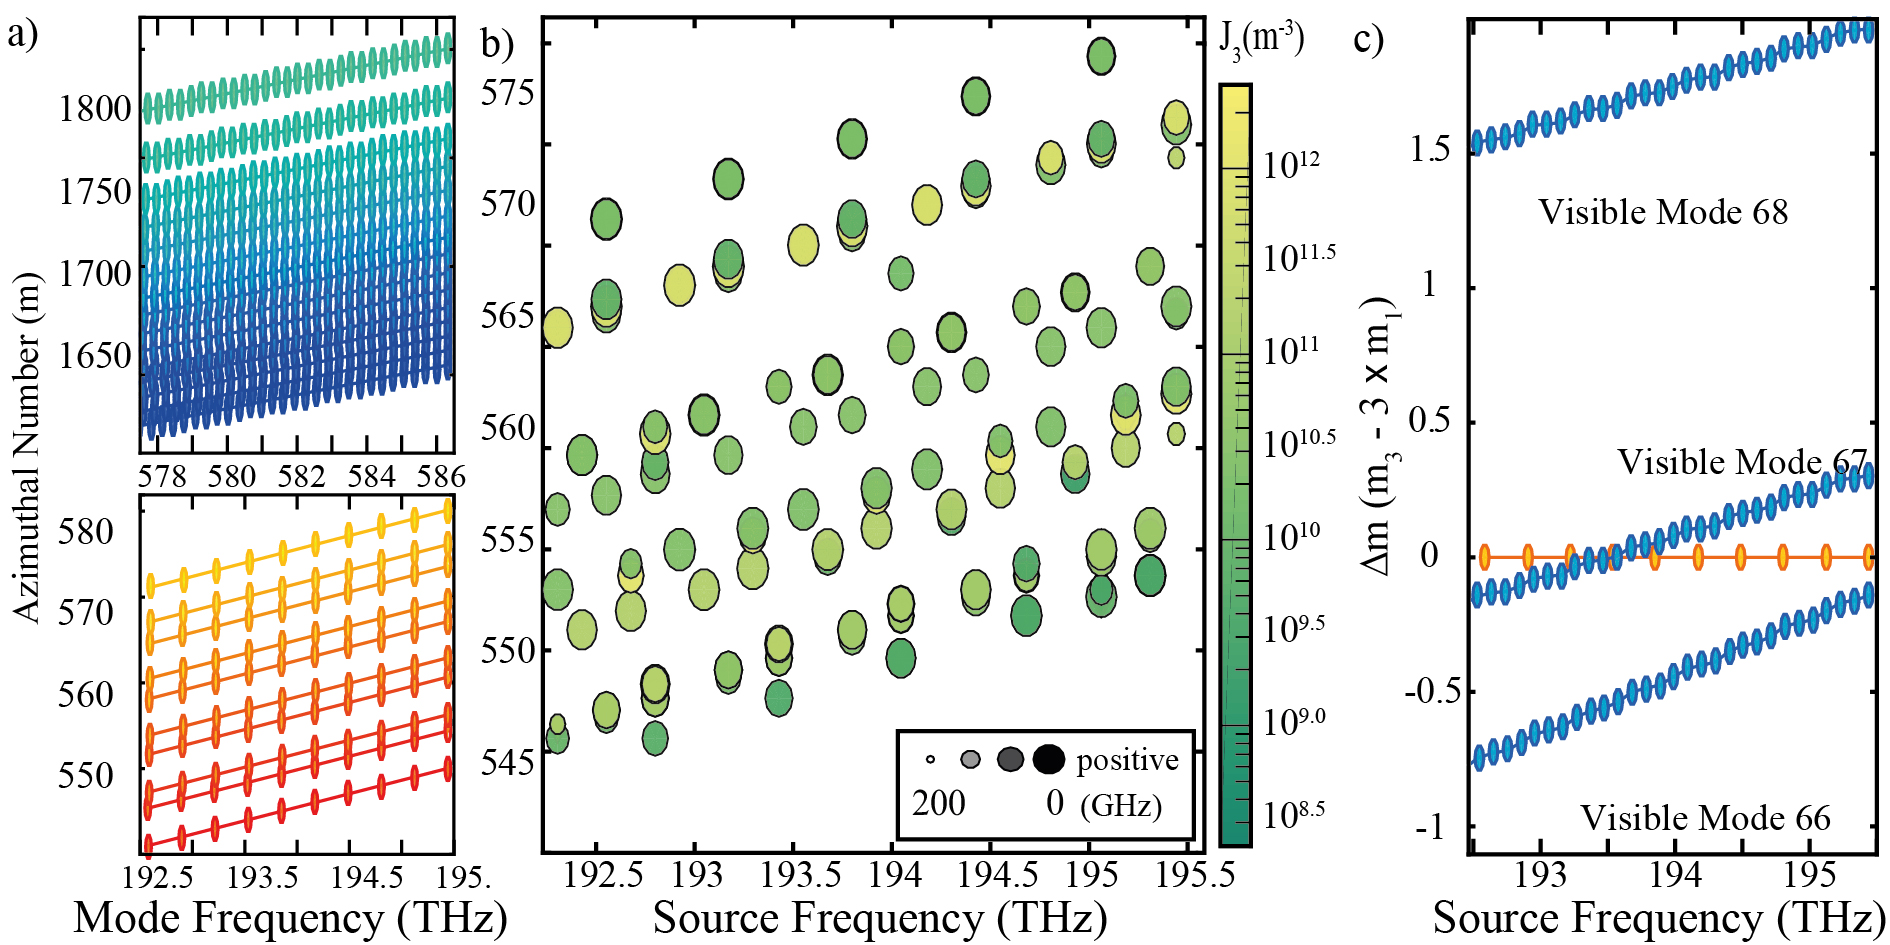
\includegraphics[width = 16cm]{figuras/Dissertation_j3_simulation.jpg}
    \caption{\textbf{Mode Simulation: a)} Simulated dispersion, upper for the visible modes and bottom the infrared modes. \textbf{b)} Calculated $J_3$ between modes that satisfy $3\times m_1 = m_3$. The color scale represents the calculated value and the size of the points correspond to the detuning between the modes. \textbf{c)} Difference between the azimuthal number of various visible modes and one infrared mode. As the source band is limited, the numbers of modes that satisfy $3\times m_1 = m_3$ for one infrared mode is small, typically one or two. }
    \label{fig:j3_sim}
\end{figure}

The simulation was made using the software COMSOL\regmark. Initially we calculate the dispersion of group of modes (10 modes for infrared and 100 for visible), the figure Fig.~\subref{fig:j3_sim}{a} shows the result  with fewer modes in the visible to facilitate the observation. We could calculate the Coupling Term between all of this modes, leading to a 10$\times$100 matrix; however, most of the pair of modes can not coupling due to the phase matching condition. To filter we must assume that $3\times m_1 = m_3$. The result is shown in Fig.~\subref{fig:j3_sim}{b}, the color map represents the value of $J_3$, and the dot size is inversely proportional of the detuning between the modes ($|\omega_3$ - $\omega_1|$). We find that the value of the overlap integral $J_3$ lies between $10^{8.5}$ and $10^{12}$ for modes that satisfy $3\times m_1 = m_3$. 

Another information that can be take from the simulation came from the calculation of the difference of the azimuthal number $\Delta m = m_3 - 3\times m_1$, shown in Fig.~\subref{fig:j3_sim}{c}. We can notice that, for a fixed infrared modes, there is few visible mode that can satisfy the phase matching.   

Now that we have all information in hand, we can measure the efficiency of THG and compare with a theoretical estimation. 

\section{Third Harmonic Generation Efficiency}
A important condition in the theoretical model is the absence of the SPM and XPM terms. To reach this condition experimentally we vary the temperature of the sample for a fixed input power. Fixing the power, the displacement of the mode due to optical bistability is fixed enabling to compensate this displacement by thermal shifting the mode, as discussed previously in Chapter~\ref{chap:couple_mode}. The Fig.~\ref{fig:max_thg} show the collected visible power for different values of temperature and input power.
\begin{figure}[h]
    \centering
    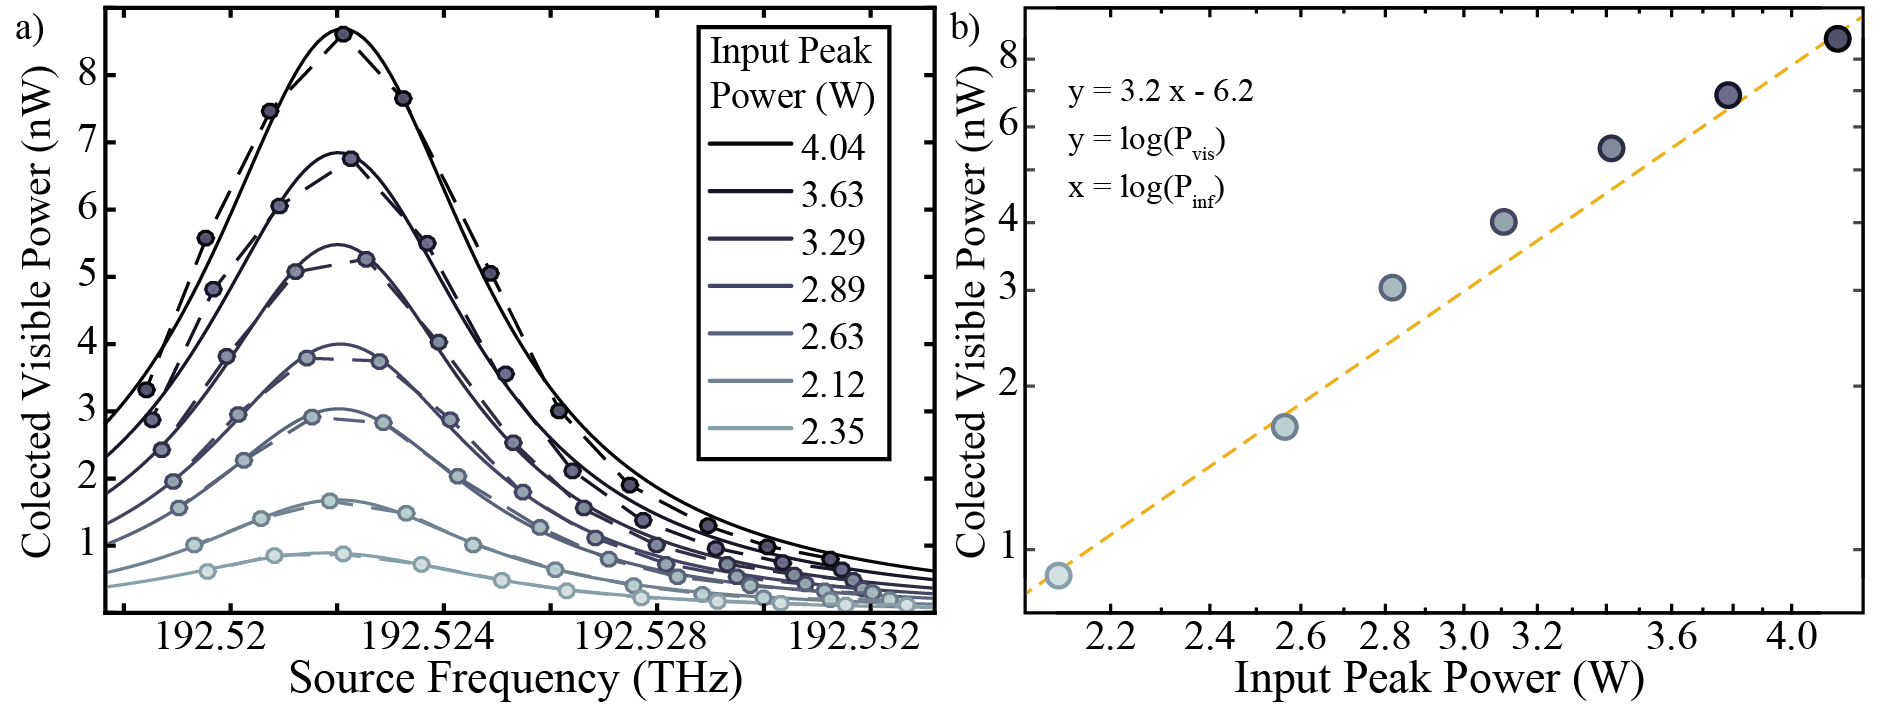
\includegraphics[width = 16cm]{figuras/Dissertation_max_thg.jpg}
    \caption{\textbf{Maximum Collected Visible power: a)} Each dot represents the maximum visible power for a fixed power and temperature. The dots with same input power was fitted to determine the maximum collected visible power. \textbf{b)} Maximum collected visible mean power in function of the input peak power in a loglog scale}
    \label{fig:max_thg}
\end{figure}

The maximum of each curve was fitted in function of the laser frequency, the fit was used to determine the maximum third harmonic generated for a fixed power. The net efficiency was defined as the ratio between the peak input power and the collected visible power divided by the duty cycle. Due to power limitation it wasn't possible to reach the region of maximum efficiency described in Chapter~\ref{chap:couple_mode}. The Fig.~\ref{fig:net_eff} compare the experimental result with the theoretical model, using the estimated values obtained in the experiments. 
\begin{figure}[h]
    \centering
    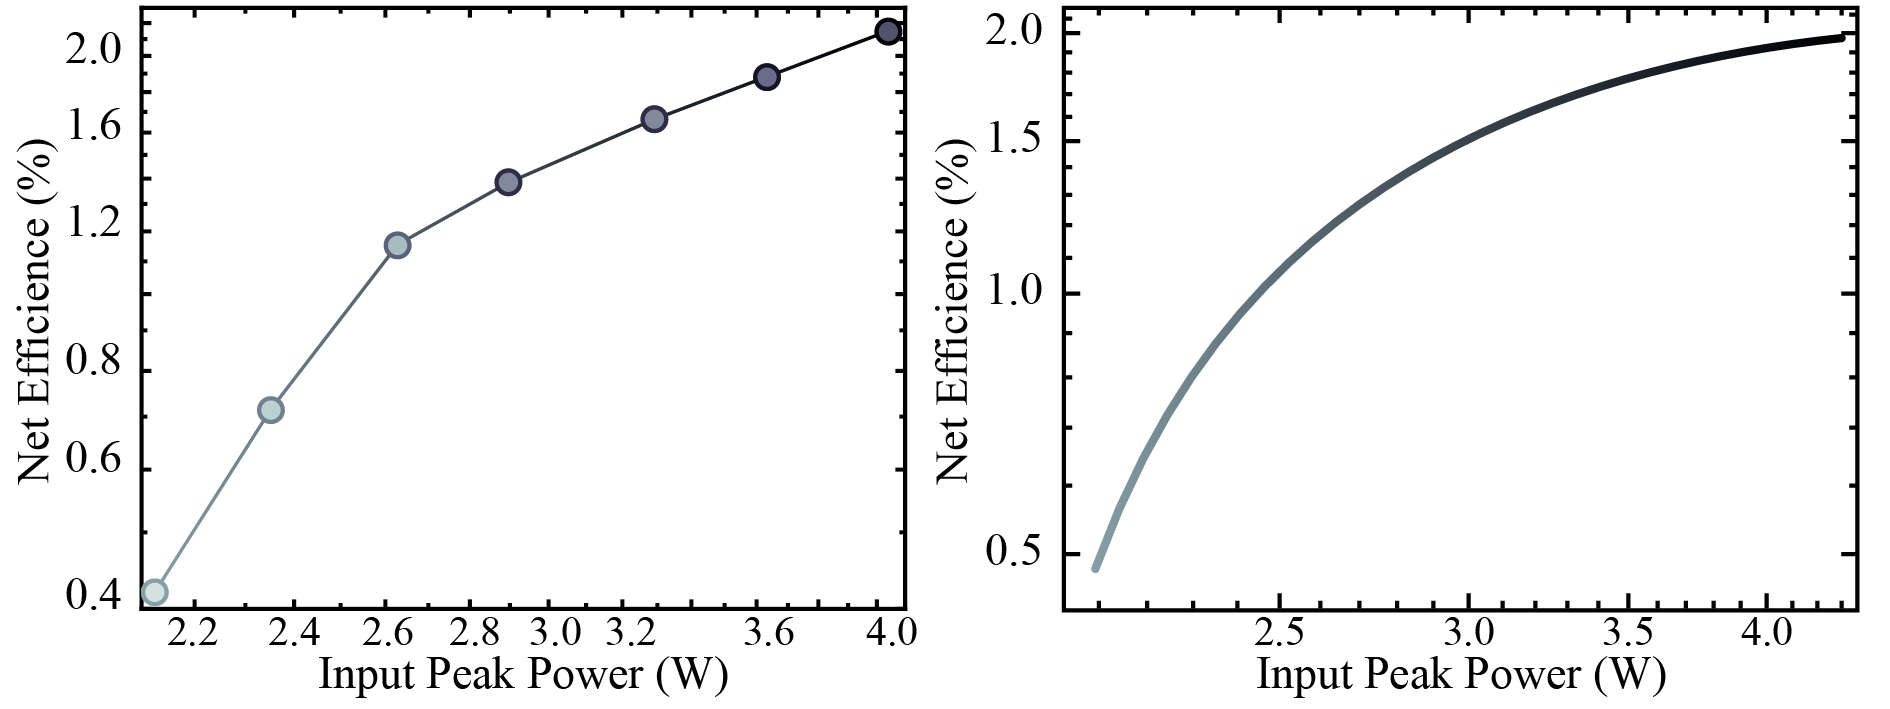
\includegraphics[width = 16cm]{figuras/Dissertation_net_eff.jpg}
    \caption{\textbf{Third Harmonic Generation Net Efficiency: a)} Efficiency, in percentage, of conversion from infrared power to visible power, experimentally measured. \textbf{b)} Theoretical model of conversion efficiency for THG.}
    \label{fig:net_eff}
\end{figure}

\section{Conclusion}

It was demonstrated Third Harmonic Generation in microcavity base on silica in a broad band. The generated light was collected using the same bus guide than the one used to pump the cavity, which facilitates the integration of the device in a optical circuit~citeCLEO.

We obtained consistent results with both techniques applied in the characterization of the visible mode, it was possible to conclude that the coupling between the visible mode and the taper is low which decrease the maximum possible net efficiency of THG. The use of a tapered optical fiber designed for visible mode was already demonstrated as a possible solution to improve the collection of visible light~\needcit.

The model proved to be compatible with the experimental result, not only to qualitatively describe the unconventional shape of the collected visible power in function of the source frequency, but also to quantitatively describe the cavity behavior. At the end of the experiment, and the project, it was possible to detect a series of improvements that can be take, it will be discussed in the next, and last, chapter.

